  %%%%%%%%%%%%%%%%%%%%%%%%%%%%%%%%%%%%%%%%%%%%%%%%%%%%%%%%%%%%%%%%%%%%%%
% LaTeX Example: Project Report

%%% Preamble
\documentclass[paper=a4, fontsize=11pt, abstract=on]{scrartcl}
\usepackage[T1]{fontenc}
\usepackage{fourier}
\usepackage{tabularx}
\usepackage[utf8]{inputenc}
\usepackage{hyperref}





\usepackage{listings}
\usepackage{color}

\definecolor{dkgreen}{rgb}{0,0.6,0}
\definecolor{gray}{rgb}{0.5,0.5,0.5}
\definecolor{mauve}{rgb}{0.58,0,0.82}
\lstset{frame=tb,
  language=[Visual]C++,
  aboveskip=3mm,
  belowskip=3mm,
  showstringspaces=false,
  columns=flexible,
  basicstyle={\small\ttfamily},
  numbers=none,
  numberstyle=\tiny\color{gray},
  keywordstyle=\color{blue},
  commentstyle=\color{dkgreen},
  stringstyle=\color{mauve},
  breaklines=true,
  breakatwhitespace=true,
  tabsize=3
}
\usepackage{graphicx}
\usepackage{caption}
\usepackage{subcaption}

\usepackage[english]{babel}															% English language/hyphenation
\usepackage[protrusion=true,expansion=true]{microtype}	
\usepackage{amsmath,amsfonts,amsthm} % Math packages

\usepackage{url}
%\usepackage[hang, small,labelfont=bf,up,textfont=it,up]{caption}


%%% Custom sectioning
\usepackage{sectsty}
\allsectionsfont{\normalfont\scshape}
\usepackage{float}
\usepackage{amsmath}
\usepackage{mathtools}
\usepackage{ragged2e}

\usepackage{nomencl}
\makenomenclature

%%% Custom headers/footers (fancyhdr package)
\usepackage{fancyhdr}
\pagestyle{fancyplain}
\fancyhead{}											% No page header
\fancyfoot[L]{}											% Empty 
\fancyfoot[C]{}											% Empty
\fancyfoot[R]{\thepage}									% Pagenumbering
\renewcommand{\headrulewidth}{0pt}			% Remove header underlines
\renewcommand{\footrulewidth}{0pt}				% Remove footer underlines
\setlength{\headheight}{13.6pt}
   \renewcommand*\abstractname{Summary}

%%% Equation and float numbering
\numberwithin{equation}{section}		% Equationnumbering: section.eq#
\numberwithin{figure}{section}			% Figurenumbering: section.fig#
\numberwithin{table}{section}				% Tablenumbering: section.tab#


%%% Maketitle metadata

\newcommand{\horrule}[1]{\rule{\linewidth}{#1}} 	% Horizontal rule

\title{
		%\vspace{-1in} 	
		\usefont{OT1}{bch}{b}{n}
		\normalfont \normalsize \textsc{} \\ [25pt]
		
\includegraphics[width=0.3\linewidth]{ubc.png} \\
		%
\includegraphics[width=0.4\linewidth]{tru}		
		\horrule{0.5pt} \\[0.2cm]
		\huge Programming Assignment \#3 : Solving Incompressible Energy Equation  \\
		\horrule{2pt} \\[0.005cm]
}
\author{
		\normalfont 								\normalsize
        Jerin Roberts\\[-5pt]		\normalsize
        \today
}
\date{}




%%% Begin document
\begin{document}
\maketitle
\begin{center}
\begin{tabular}{l r}


Supervisor: & Dr. Carl Ollivier-Gooch  \\ % supervisor
Locations: & University of British Columbia


\end{tabular}
\end{center}



\newpage
\tableofcontents
\listoffigures
\listoftables
\newpage
\lstset{language=[Visual]C++}
\section{Introduction}



 The are many physical phenomenons in physics and engineering that require linear and non-linear partial differential equations to described the true nature of the system. Solving these systems analytically and finding exact solutions for these equations can be difficult and often require simplifications that ultimately don't fully represent the problem being investigated. Numerical methods for solving PDE's provides a means for finding approximations to the exact solutions without having to make sacrificial simplifications. With recent advancements in computational technology numerical methods can now be easily applied to large and difficult problems that would otherwise be impossible to solve. 
\subsection{Problem Overview}
Numerical problems are essentially solved by breaking the entire solution domain into small discrete points (mesh) and finding the solution at or around these areas. Each point requires the solving the differential equations that represent physical phenomenon being investigated. Since the exact solution cannot be computed, it is instead approximated using various techniques and methods. In this assignment the 2D in-compressible laminar energy equation is applied to a rectangular channel for a given velocity field. The problem will employ an second ordered centered flux calculation with both implicit and explicit euler timer advance methods. The implicit method will be solved using approximate factorization and Gauss-Jordan elimination via the Thomas algorithm. Boundary conditions will be implement using ghost cells allowing the interior scheme to remain the same during calculation of bordering cells. The ghost cells are calculated such the boundary condition is enforced at $i=1/2$.



\section{Implementation}
\subsection{Program Overview}
The C/C++language was selected for this programming assignment. The scripts were compiled using g++/gcc version 5.4.0 on Ubuntu 16.04.02 and are available in the attached zip or for clone via the link provided: \url{https://github.com/j16out/cfd510} . The program itself is broken into 3 pieces and two levels to produce a modular set that makes it easier to apply to different problems. The highest level contains the "macro" or the main function which can be modified for different problems. 
The numerical directory contains numerical.cpp script and its header file numerical.hpp. This set contains all the functions necessary for solving the problem numerically. The appendix contains the .hpp file which lists all functions with a short description of each. The vroot directory contains the scripts necessary for drawing data. These scripts make use of the ROOT-v6 libraries. ROOT is a popular data analysis framework primarily written in C++ and Phython. For more information on ROOT libraries visit the link provided: \url{https://root.cern.ch/} .

 
\subsection{Solution Method}
There are three general routes that can be taken to solve the Navier-Stokes equations each of which is characterized by the way it satisfies the continuity equation; Stream function-vorticity methods take and express the velocity field in terms of derivatives of the stream function. Because of this the momentum equations are replaced by a single vorticity transport equation, while a Poisson equation relates the stream function and vorticity.  This method works fine for 2D flows, but can be difficult to use in three dimensions as stream function is a 2D entity. The 2nd type is Pressure Poisson methods, which take the divergence of the momentum equations and manipulate this to get a Poisson equation for the pressure. This equation can be simplified by using the continuity equation to eliminate terms. These methods are well-known in the field, but have a reputation for being difficult to program. The method selected for this project is the artificial compressibility method. This method adds a physical time derivative of pressure to the continuity equation. This derivative is scaled by a parameter $\beta$ that effectively sets the pseudo-compressibility of the fluid.The addition of a
time derivative of pressure enables the coupling of the continuity equation with the
momentum equations which ideally allows us to advance pressure and velocity in time
together.

The non-dimensional Navier-Stokes equations in
artificial compressibility form can be written as equations \ref{gov1} to \ref{gov2}

\begin{equation}
\label{gov1}
\frac{\partial P}{\partial t}+\frac{1}{\beta}\frac{\partial u}{\partial x}+\frac{1}{\beta}\frac{\partial v}{\partial y} = 0
\end{equation} 

 \begin{equation}
\label{nav}
\frac{\partial u}{\partial t} +\frac{\partial u^2}{\partial x}+\frac{\partial vu}{\partial y} = -\frac{\partial P}{\partial x} + \frac{1}{Re} \Bigg(  \frac{\partial^2 u}{\partial x^2} + \frac{\partial^2 u}{\partial y^2} \Bigg)
\end{equation} 

 \begin{equation}
\label{gov2}
\frac{\partial v}{\partial t} +\frac{\partial vu}{\partial x}+\frac{\partial v^2}{\partial y} = -\frac{\partial P}{\partial y} + \frac{1}{Re} \Bigg(  \frac{\partial^2 v}{\partial x^2} + \frac{\partial^2 v}{\partial y^2} \Bigg)
\end{equation} 

We can take this and write it in our standard form (eq \ref{stand} which enables to integrate over the computational cell by applying gauss's Theorem and dividing over the size of the finite volume.

 \begin{equation}
\label{stand}
\frac{\partial U}{\partial t} + \frac{\partial F}{\partial x} + \frac{\partial G}{\partial y} = 0
\end{equation} 

where

\begin{equation}
\label{nav2}
U= \begin{bmatrix}
   P    \\
   u  \\
    v
\end{bmatrix}
\end{equation} 

\begin{equation}
\label{nav3}
F= \begin{bmatrix}
    \frac{u}{\beta}    \\
   u^2+P-\frac{1}{Re}\frac{\partial u}{\partial x}  \\
    uv-\frac{1}{Re}\frac{\partial v}{\partial x}
\end{bmatrix}
\end{equation} 


\begin{equation}
\label{nav4}
G= \begin{bmatrix}
    \frac{v}{\beta}    \\
   uv-\frac{1}{Re}\frac{\partial u}{\partial y} \\
    v^2+P-\frac{1}{Re}\frac{\partial v}{\partial y} 
\end{bmatrix}
\end{equation} 
Which leads to navier stokes in finite volume form as shown in equation \ref{fv}


\begin{equation}
\label{fv}
\frac{d U_{ij}}{d t} = -\frac{F_{i+\frac{1}{2},j}-F_{i-\frac{1}{2},j}}{\triangle x} -\frac{G_{i, j+\frac{1}{2}}-G_{i,j-\frac{1}{2}}}{\triangle y}
\end{equation} 

Where the right hand side (RHS) represents the 2nd order approximation to the flux integral, where U, G, and F as before are represented as 3x1 matrices of Pressure and velocity components.
\section{Validation}
\subsection{Flux Computation}

 The program was built and tested in small components to ensure its correctness. The flux integral was run and compared to the exact solution for the flux integral. The problem will employ a second ordered centered flux calculation which is found on the RHS of the discretized energy equation.


The flux was calculated using the function $update\_ flux()$, which is shown below. The function calls two other functions which grab the necessary data using the $surr$ struct from the current solution. The flux calculated using $calc\_ newcell()$ is then stored on the $carray$ struct under the $f1$ array.

\begin{lstlisting}
void update_flux(carray & myarray){
surr mysurr;
vec ftemp;
for(int j = 1; j < myarray.sizey-1; ++j)
{
    for(int i = 1; i < myarray.sizex-1; ++i)
    {
    //----get surrounding cells and compute new cell----//
    get_nsurcells(myarray, i, j, mysurr);    
    calc_flux(myarray, mysurr, ftemp); 
    
    //-----update current cell----//  
    myarray.f1[i][j] = ftemp;   
    }
}
}
\end{lstlisting}




The correctness of the flux integral was validated using the exact computed flux. The $L_2$ norms for the flux calculation are displayed in table \ref{norm1}. The order of accuracy for the scheme was determined using the log log method as displayed in figure \ref{fluxo}. The order of accuracy for this scheme was estimated to be 2nd order accurate based on the $L_2$ data from 8 different meshes.     
    
  

\begin{figure}[H]
\centering
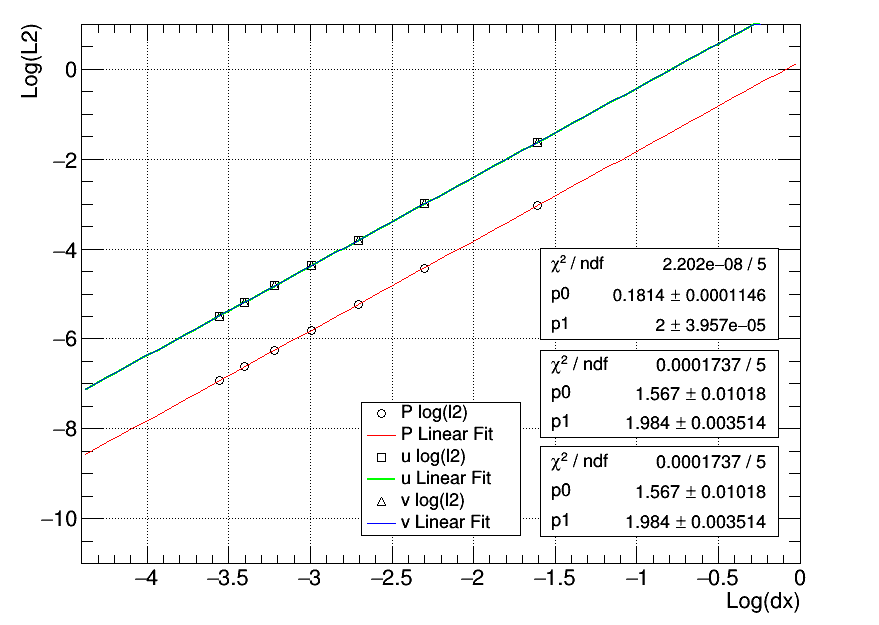
\includegraphics[width=0.75\linewidth]{flux}
\caption{Order of Accuracy of Flux Integral for Pressure and Velocity components}
\label{fluxo}
\end{figure}



\begin{table}[H]
\begin{center}
    \begin{tabular}{ | p{0.13\linewidth} | p{0.2\linewidth} |p{0.2\linewidth} |p{0.1\linewidth} |p{0.1\linewidth} |p{0.1\linewidth} |}
 \hline  
     \RaggedRight \textbf{Mesh Size}
    &\RaggedRight \textbf{Pressure $L^2$norm}
    &\RaggedRight \textbf{Velocity $L^2$norm}
    &\RaggedRight \textbf{$\triangle x$}
    &\RaggedRight \textbf{Order}
    \\ \hline  
           \RaggedRight 10 x 10
    &\RaggedRight 4.7946 $*10^{-2}$
    &\RaggedRight 1.9505 $*10^{-1}$
    &\RaggedRight 0.1
    &\RaggedRight -
    \\ \hline 
    \RaggedRight 20 x 20
    &\RaggedRight 1.1983 $*10^{-2}$
    &\RaggedRight 5.0025 $*10^{-2}$
    &\RaggedRight 0.05
    &\RaggedRight 1.952
    \\ \hline 
           \RaggedRight 40 x 40
    &\RaggedRight 2.9957  $*10^{-3}$
    &\RaggedRight 1.2585  $*10^{-2}$
    &\RaggedRight 0.025
    &\RaggedRight 1.980
    \\ \hline 
           \RaggedRight 80 x 80
    &\RaggedRight 7.4892 $*10^{-4}$
    &\RaggedRight 3.1514 $*10^{-3}$
    &\RaggedRight 0.0125
    &\RaggedRight 2.002
    \\ \hline       
   \end{tabular}
\end{center} 
\caption{Table of $L^2$ norms for increasing mesh size of flux integral for RHS}
\label{norm1} 
\end{table}

This matches what was expect by implementing a 2nd order interior flux evaluation and boundary schemes. It should be noted as seen in figure \ref{fluxo} the error decreases when refining the mesh. This is expect as the numerical solution is a discrete representation of the continuous exact solution. 

 
\subsection{Flux Jacobian}
For the time discetization of the Navier-Stokes equations a implicit euler method was selected. The fully implicit time discretization of NS equations can be written as 


 \begin{equation}
  \begin{aligned}
\delta U_{ij} + \triangle t A_x \delta U_{i-1,j} + \triangle t B_x \delta U_{i,j} + \triangle t C_x \delta U_{i+1,j}\\
  +\triangle t A_y \delta U_{i,j-1} + \triangle t B_y \delta U_{i,j} + \triangle t A_y \delta U_{i,j+1} \\
  = -\triangle t \frac{F_{i+\frac{1}{2},j}-F_{i-\frac{1}{2},j}}{\triangle x} -\triangle t \frac{G_{i, j+\frac{1}{2}}-G_{i,j-\frac{1}{2}}}{\triangle y}
 \end{aligned}
\end{equation}

The implementation of the left hand side (LHS) can be validated by implementing a very small known change in solution for one cell between time steps. The difference between the flux calculated on the RHS from time level n to n+1 should be roughly equivalent to the LHS of the implementation (minus $\delta U_{ij}$). 



 \begin{equation}
  \begin{aligned}
 \Bigg( \frac{F_{i+\frac{1}{2},j}-F_{i-\frac{1}{2},j}}{\triangle x} - \frac{G_{i, j+\frac{1}{2}}-G_{i,j-\frac{1}{2}}}{\triangle y}\Bigg)^{n+1}
  \\ -\Bigg( \frac{F_{i+\frac{1}{2},j}-F_{i-\frac{1}{2},j}}{\triangle x} - \frac{G_{i, j+\frac{1}{2}}-G_{i,j-\frac{1}{2}}}{\triangle y}\Bigg)^{n} \\
   = A_x \delta U_{i-1,j} +  B_x \delta U_{i,j} +  C_x \delta U_{i+1,j}\\
  + A_y \delta U_{i,j-1} +  B_y \delta U_{i,j} +  A_y \delta U_{i,j+1}
 \end{aligned}
\end{equation}


Since we've only selected one cell to change only 5 cells in total will see a calculated change which corresponds each to one term on the LHS being non-zero. This provides a great method for narrowing down which term was incorrect. If the error was found to be greater then $10^{-10}$ then the term was considered to be incorrect. The errors for each corresponding component of change are tabulated in table \ref{tLHS}.

\begin{table}[H]
\begin{center}
    \begin{tabular}{ | p{0.2\linewidth} | p{0.2\linewidth} |p{0.2\linewidth} |p{0.2\linewidth}| }
 \hline  
     \RaggedRight \textbf{Component (i, j)}
    &\RaggedRight \textbf{Pressure Error}
    &\RaggedRight \textbf{u Error}
    &\RaggedRight \textbf{v Error}
    \\ \hline  
           \RaggedRight Ax (11, 10)
    &\RaggedRight 3.000 $*10^{-15}$
    &\RaggedRight 5.001 $*10^{-12}$
    &\RaggedRight 5.001  $*10^{-12}$
    \\ \hline 
    \RaggedRight Cx (9, 10)
    &\RaggedRight 1.000 $*10^{-15}$
    &\RaggedRight 5.002 $*10^{-12}$
    &\RaggedRight 5.001  $*10^{-12}$
    \\ \hline 
           \RaggedRight Bx By (10, 10)
    &\RaggedRight 1.000  $*10^{-15}$
    &\RaggedRight 2.500  $*10^{-13}$
    &\RaggedRight 2.500  $*10^{-13}$
    \\ \hline 
           \RaggedRight Cy (10, 9)
    &\RaggedRight 1.000 $*10^{-15}$
    &\RaggedRight 5.001 $*10^{-12}$
    &\RaggedRight 5.000 $*10^{-12}$
    \\ \hline       
           \RaggedRight Ay (10, 11)
    &\RaggedRight 3.000 $*10^{-15}$
    &\RaggedRight 4.995 $*10^{-12}$
    &\RaggedRight 4.995 $*10^{-12}$
    \\ \hline    
   \end{tabular}
\end{center} 
\caption{Table of $L^2$ norms for increasing mesh size of flux integral}
\label{tLHS} 
\end{table}

\subsection{Block Thomas}



\begin{lstlisting}
void solve_LinSys(carray & myarray, double tstep, double & mdiff)
{
//--linear system num 1---//
crow myrow;
for(int j = 1; j < myarray.sizey-1; ++j)
{
load_row(myarray, myrow, j, tstep);
solve_block_thomas(myarray, myrow, myarray.sizex, j);
}
ccol mycol;
for(int i = 1; i < myarray.sizex-1; ++i)
{
load_col(myarray, mycol, i, tstep);
solve_block_thomas(myarray, mycol, myarray.sizey, i);
}
}

\end{lstlisting}

\subsection{Boundary Conditions}
The boundary condition are divided into twotypes; explicit and implicit. The explicit ones are used to enforce the boundary conditions during the flux calculation for the RHS. They are set using the $set\_ghost\_cell()$ function which is displayed below. For this problem only wall boundaries are used
\subsection{Pressure Oscillations}
It was found that steady-state pressure distributions have
some oscillations. These were present because of decoupling between pressure in alternate lines of the mesh. To fix this problem a term was added to the
right-hand side of the pressure equation which is displayed as \ref{osc}. 

 \begin{equation}
\label{osc}
A\Bigg(\frac{\overline{P}_{i+1,j}-2\overline{P}_{i,j}+\overline{P}_{i-1,j} }{\triangle x^2} +\frac{\overline{P}_{i,j+1}-2\overline{P}_{i,j}+\overline{P}_{i,j-1} }{\triangle y^2}\Bigg)\triangle x \triangle y
\end{equation} 
This essentially introduces an artificial component which for a properly selected $A$ can smooth out the pressure fluctuations while maintaining 2nd order accuracy.
A value of 0.01 was selected for A. The effect of the correction is displayed in figure \ref{osc2} 

\begin{figure}[H]
        \centering
        \begin{subfigure}[h]{0.5\textwidth}
                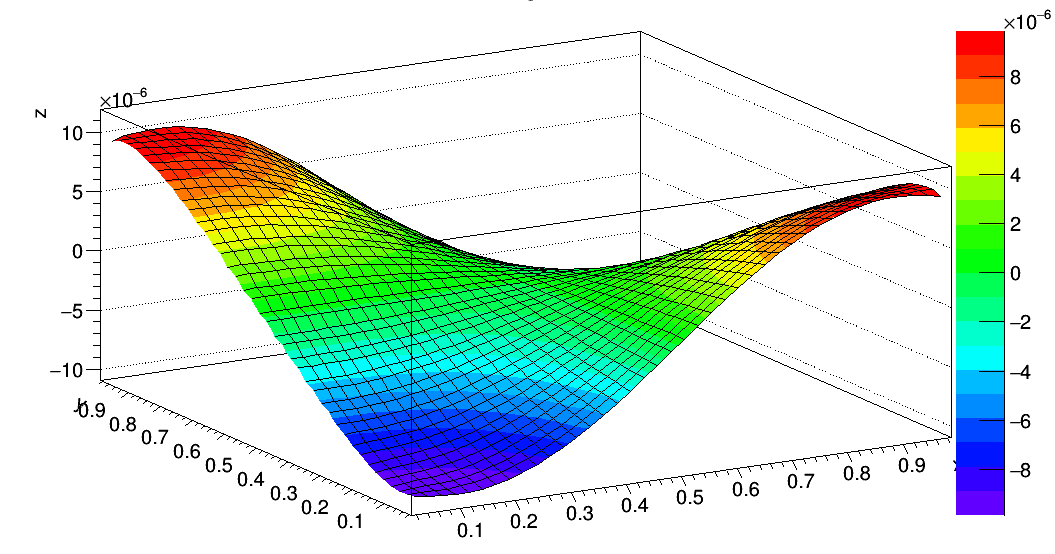
\includegraphics[width = 7.5cm]{o1}
                \caption{}
				
        \end{subfigure}%
       ~~~~~
        \begin{subfigure}[h]{0.5\textwidth}
                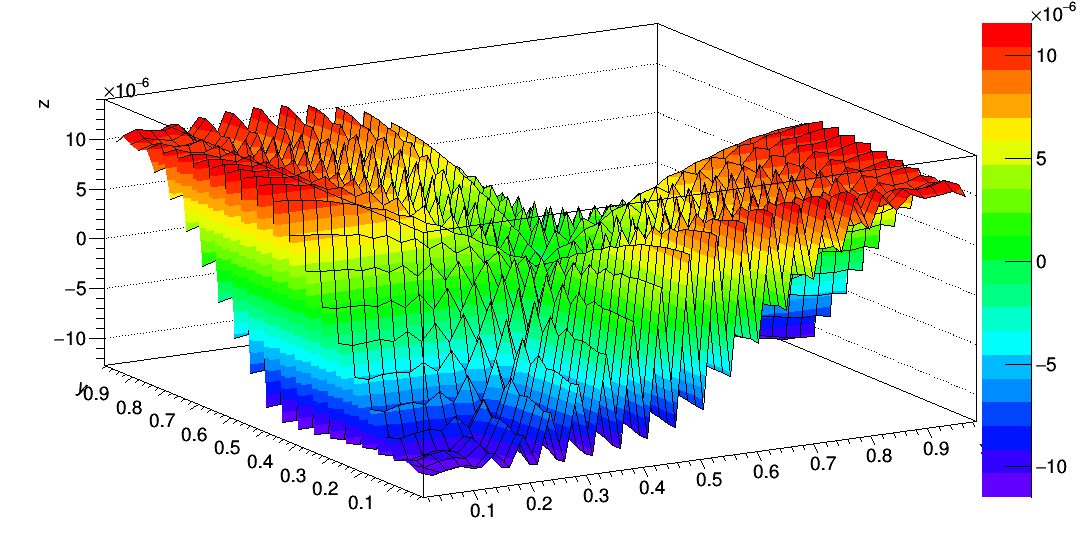
\includegraphics[width = 7.7cm]{o2}
                \caption{}
                
        \end{subfigure}
        \caption{Correcting pressure oscillations for 40x40 mesh (a) corrected A = 0.01 (b) uncorrected A = 0  }
        \label{osc2}
\end{figure}

\section{Program Testing}

\begin{figure}[H]
\centering
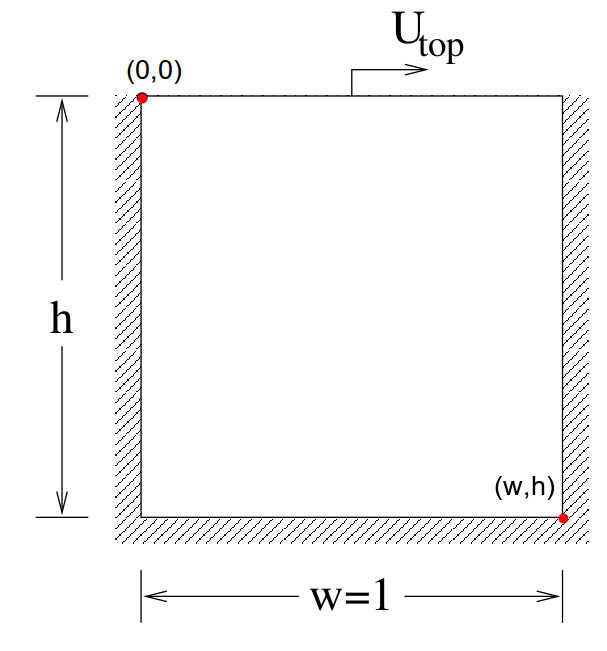
\includegraphics[width=0.65\linewidth]{box}
\caption{diagram of box modeled in problem}
\label{prob}
\end{figure}

To test the program a problem concerning the flow in an enclosed box with a
moving top was evaluated. A diagram of the problem is displayed in figure \ref{prob} The walls and the lid of the box also has a no-slip boundary condition, where the lid is at constant velocity U top. As the top of the box moves to the right, the fluid in the box circulates clockwise (for a square box). For all cases in this section a Reynolds number of 100 and $\beta = 1$ was used. The initial conditions for the problem are displayed in equation \ref{init}

\begin{equation}
\label{init}
\begin{bmatrix}
   P    \\
   u  \\
    v
\end{bmatrix} =
\begin{bmatrix}
   P_0\cos(\pi x)\cos(\pi y)   \\
   u_0\sin(\pi x)\sin(2\pi y)  \\
    v_0\sin(2\pi x)\sin(\pi y)
\end{bmatrix}
\end{equation} 
The origin for the computational domain is set at top left corner of box. Therefore the lid is found along the y=0 plane which will be the convention for the remainder of report.
\subsection{Stability}
For stability test the top plate velocity was set to zero and the problem was solve to steady state. The convergence was logged for each iteration, its history is displayed in figure \ref{con}. A 20x20 mesh was used with a 0.05 second time step. The convergence exhibits some oscillatory behavior which seems to be mediated through the use of larger time steps. The oscillations seen in the convergence history can physically be thought of as pressure waves bouncing around inside the domain which will inherently induce velocity changes that are out of phase with the pressure changes. The solution for pressure and velocity components converged toward zero gauge pressure and velocity which confirms the stability of the code. This is demonstrated in figures \ref{zero1} where solutions are shown approaching zero and equalizing. 




\begin{figure}[H]
        \centering
        \begin{subfigure}[h]{0.5\textwidth}
                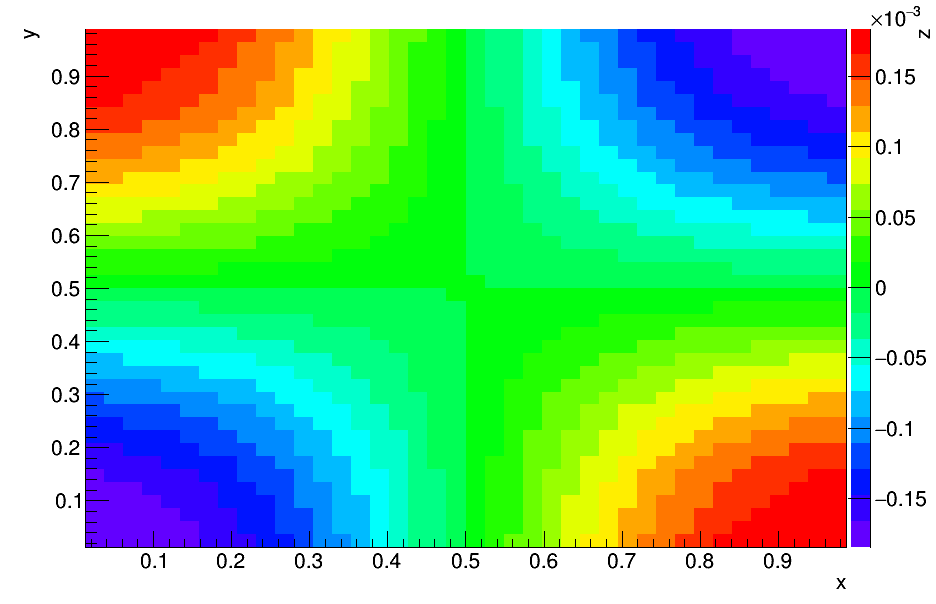
\includegraphics[width = 7.5cm]{z1}
                \caption{}
				
        \end{subfigure}%
       ~~~~~
        \begin{subfigure}[h]{0.5\textwidth}
                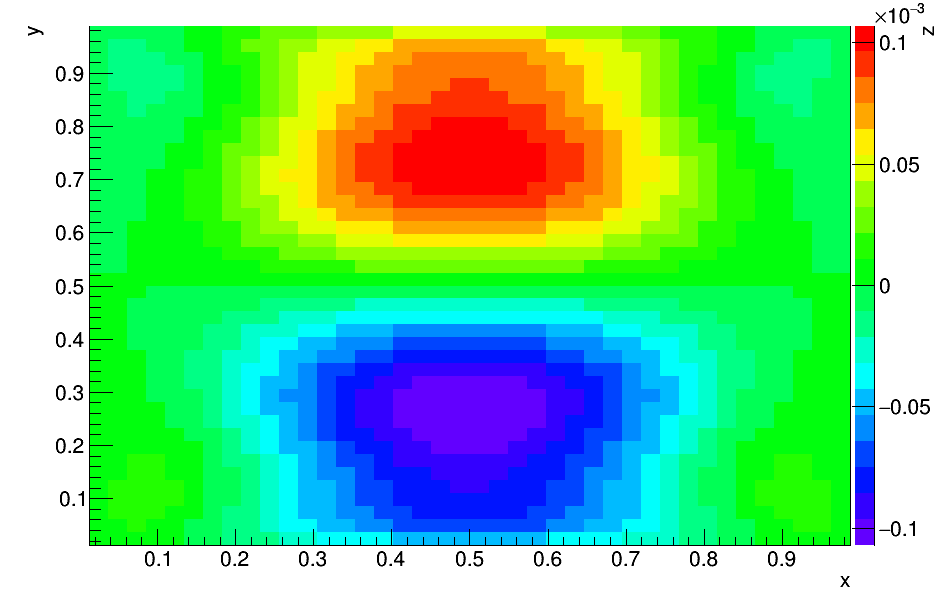
\includegraphics[width = 7.5cm]{z2}
                \caption{}
                
        \end{subfigure}
        \caption{Solutions approaching zero for Pressure (a) and Velocity u (b). Note the z scale is order $\approx 10^{-3}$ }
        \label{zero1}
\end{figure}



\begin{figure}[H]
\centering
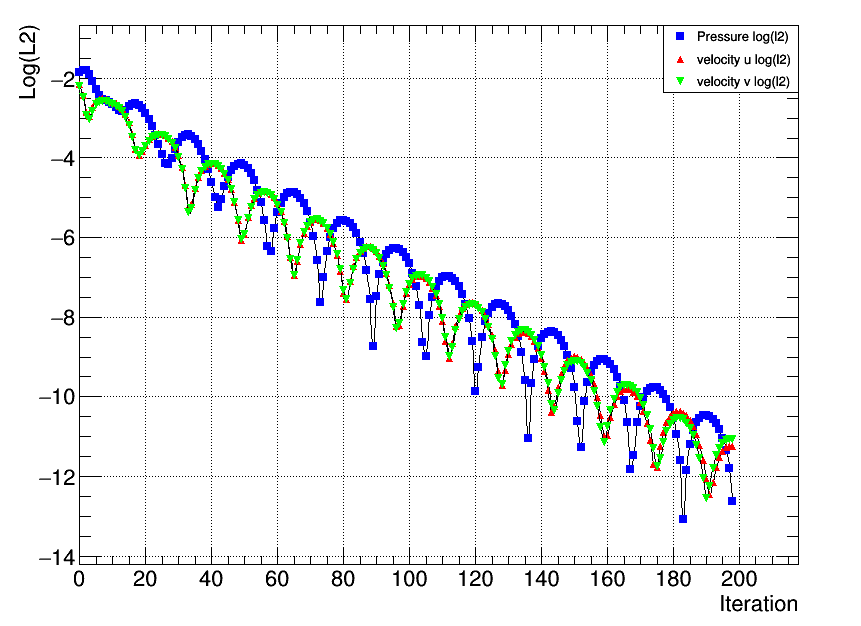
\includegraphics[width=0.80\linewidth]{stabord}
\caption{convergence history for flow inside enclosed box. }
\label{con}
\end{figure}

 

\subsection{Solution $U_{top} = 1$}
The solution for the flow inside the box was calculated when the speed of the lid was set to $U_{top} = 1$. The height was set to $h=1$ and time step set to $\triangle t = 0.1$. No over relaxation was used during this evaluation. Figure \ref{conh} displays the convergence history during the solving of the solution. Again we see oscillatory behavior which begins to smooth out as the solution refines. The velocity profile for the x-velocity u was plotted at $x=0.5$ for different values of height inside the box which displays the u-velocity along the line of vertical symmetry. Since the mesh is even value points at x = 0.5 had to be calculated using surrounding cell data.  For each y cell (row) 2 cells on each side of x = 0.5 were used (total = 4) to fit a 2nd degree polynomial function which was then used to calculate the value at $x= 0.5$. The u-velocity along the vertical line of symmetry for $U_{top} = 1$ is displayed in figure \ref{usym1}. 

\begin{figure}[H]
\centering
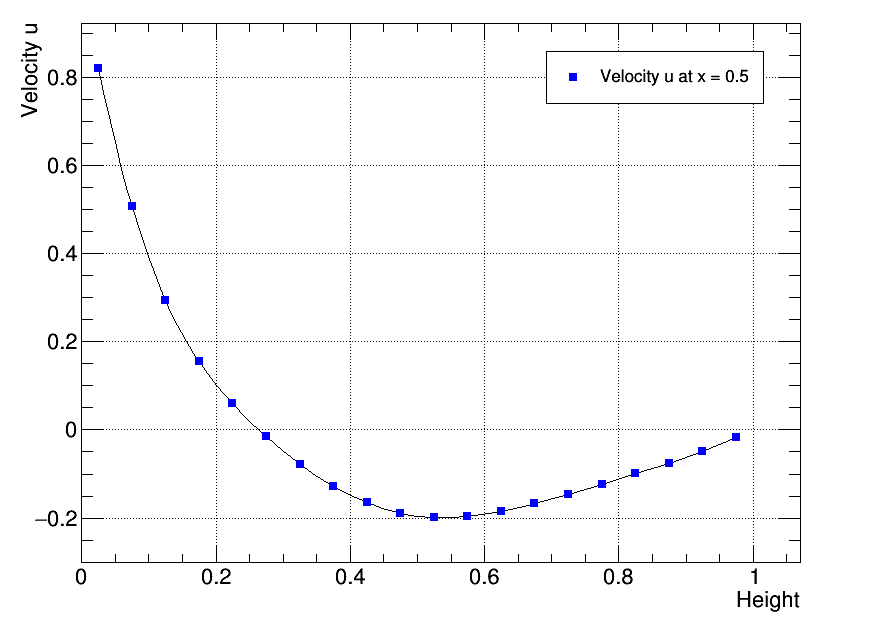
\includegraphics[width=0.80\linewidth]{con1}
\caption{Velocity u profile at x = 0.5 for $U_{top}=1$. Lid found at y = 0. }
\label{usym1}
\end{figure}


\begin{figure}[H]
        \centering
        \begin{subfigure}[h]{1.0\textwidth}
        \centering
                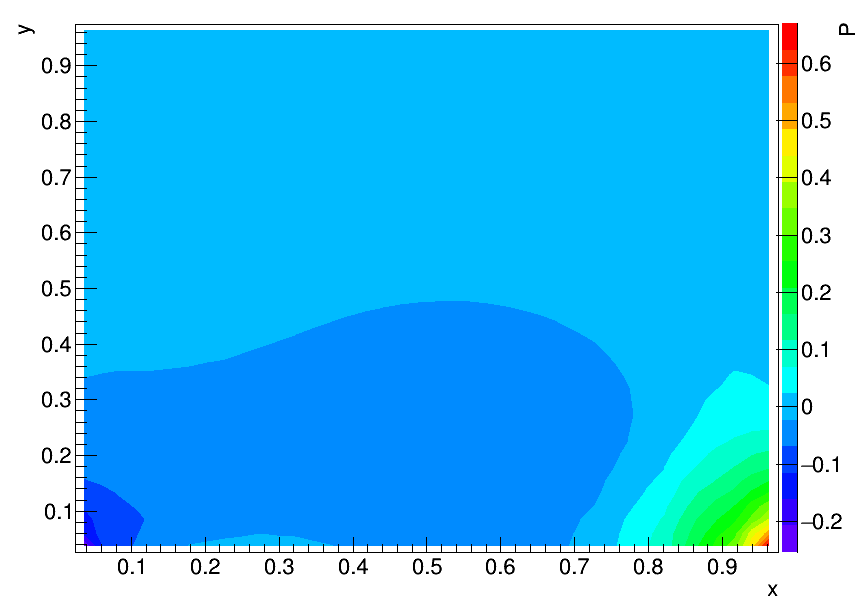
\includegraphics[width = 12.5cm]{con2}
                \caption{}
				
        \end{subfigure}%
        \newline
       \centering
        \begin{subfigure}[h]{0.9\textwidth}
        \centering
                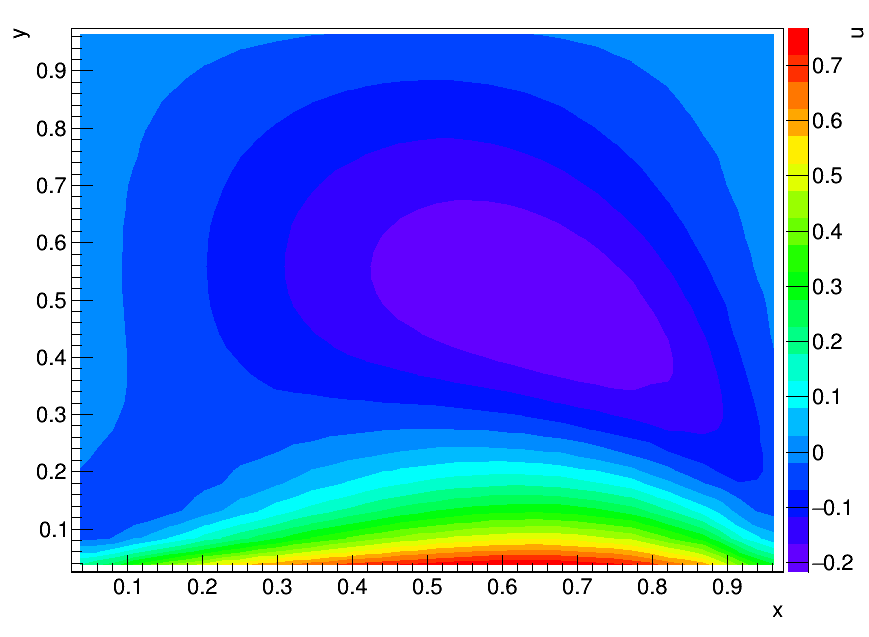
\includegraphics[width = 12.5cm]{con4}
                \caption{}
                
        \end{subfigure}
        \caption{Pressure Distribution (a) and u-Velocity (b) inside box for Solution $U_{top}=1$ and A = 0.5}
        \label{zero}
\end{figure}


\begin{figure}[H]
\centering
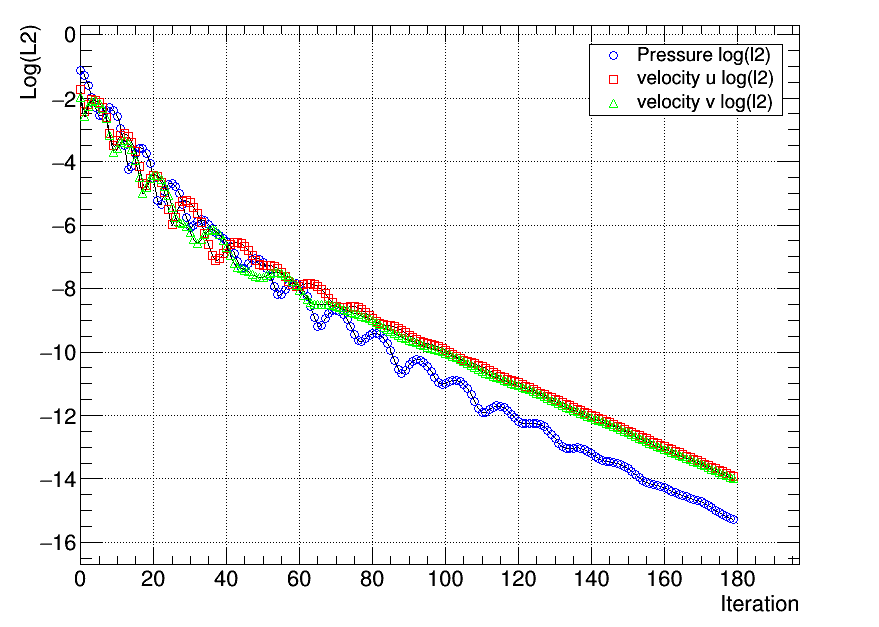
\includegraphics[width=0.80\linewidth]{con3}
\caption{convergence history of flow inside enclosed box for $\triangle t = 0.1$}
\label{conh}
\end{figure}

\subsection{Solution $U_{top} = -1$}
Additionally the solution for the flow inside the box was calculated when the speed of the lid was set to $U_{top} = -1$. The height was set to $h=1$ and time step set to $\triangle t = 0.1$. No over relaxation was used during this evaluation. This was then contrasted with the previous solution at $U_{top} = 1$ by flipping $U_{top} = -1$ over the vertical axis of symmetry and adding it to 
$U_{top} = 1$. 
\begin{figure}[H]
\centering
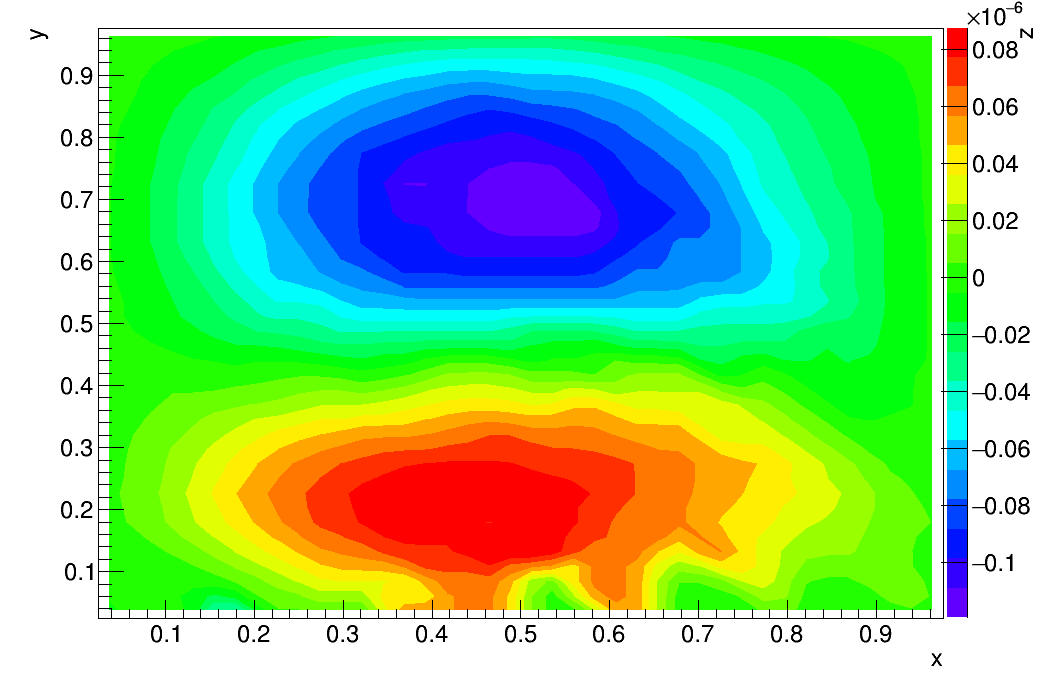
\includegraphics[width=0.80\linewidth]{sanity}
\caption{A contour of $u_{U_{top} = 1}(x,y) + u_{U_{top} = -1}(1-x,y)$ displaying the program symmetry}
\label{san1}
\end{figure}

More specifically a contour of $u_{U_{top} = 1}(x,y) + u_{U_{top} = -1}(1-x,y)$ was found and displayed in figure \ref{san1}. This shows the continuity of the program by comparing the error for opposite symmetry problems. Because the error seen is really small its attributed to a lack of iterative convergence.




\section{Vortices problem}
For the Lid-driven cavity problem the height h of the box was increased. The single vortex seen in previous examples eventually becomes unstable, and a second vortex forms below it and eventually a third, and so on. The exploratory part of this problem will focus on this formation of additional vortices with an increase in the height of the cavity. 

\subsection{Vortex Location}
When the height was increased to $h=3$ the cavity was observed to produce a total of three vortices. The vortices were discovered using a contour plot of the magnitude of the velocity components u and v. By generating a contour plot of the magnitude of u and v one could easily search out locations where the magnitude was zero, suggesting a potential area for a vortex. Figure \ref{v1} displays three vortices identified for a cavity of $h=3$.


\begin{figure}[H]
        \centering
        \begin{subfigure}[h]{0.5\textwidth}
        \centering
                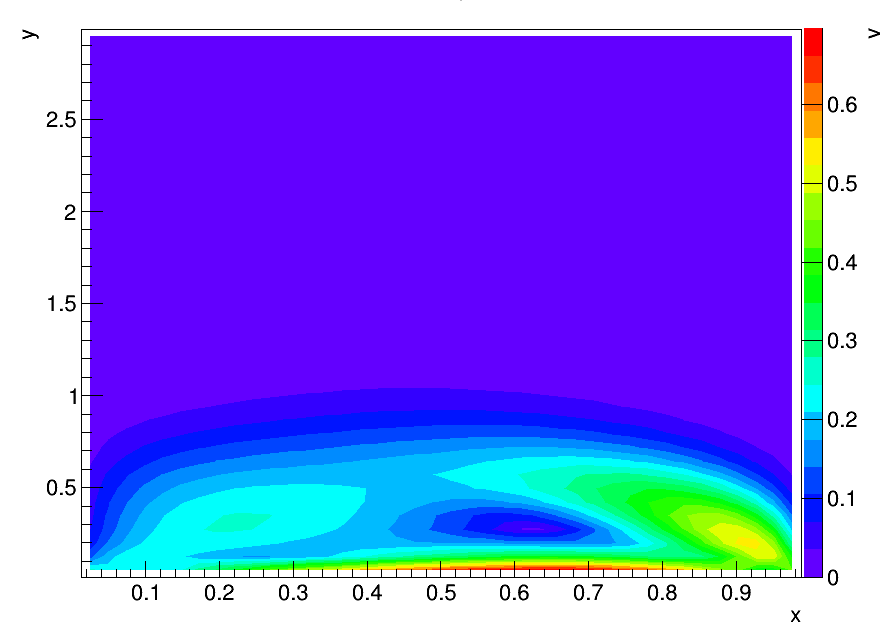
\includegraphics[width = 5.5cm]{v1}
                \caption{}				
        \end{subfigure}%
       ~~~~~
        \begin{subfigure}[h]{0.5\textwidth}
        \centering
                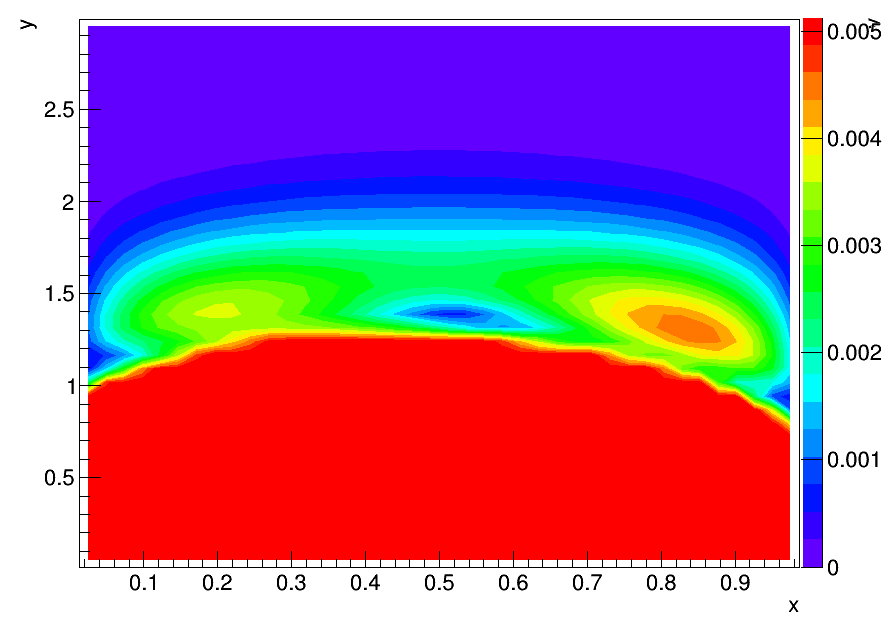
\includegraphics[width = 5.5cm]{v2}
                \caption{}               
        \end{subfigure}       
         ~~~~~
        \begin{subfigure}[h]{0.5\textwidth}
        \centering
                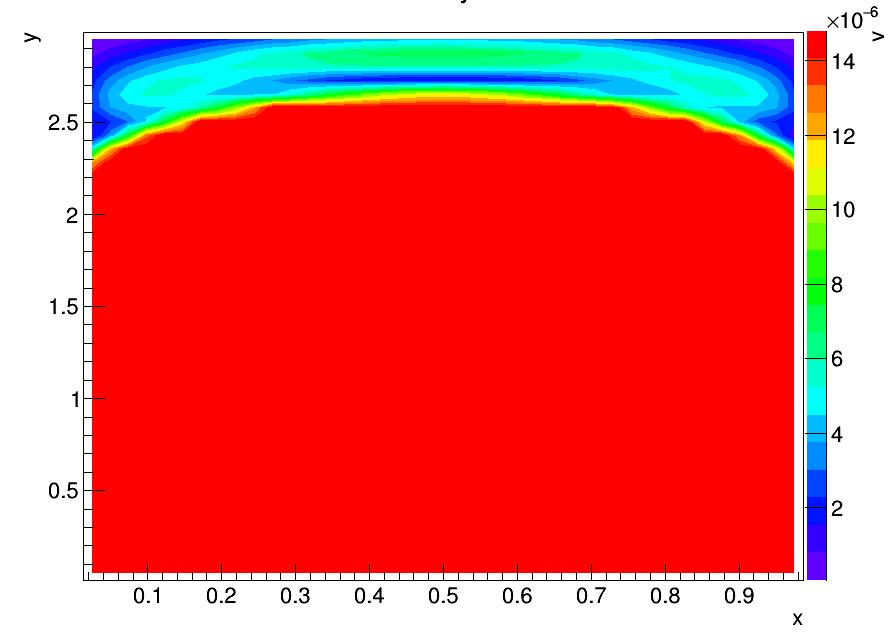
\includegraphics[width = 5.5cm]{v3}
                \caption{}               
        \end{subfigure}
        \caption{Solutions approaching zero for Pressure (a) and Velocity u (b). Note the z scale is order $\approx 10^{-3}$ }
        \label{zero1}
\end{figure}



 Once a vortex was identified a curve fitting method was employed to calculated its center. The method works by approximating the dip in velocity magnitude or the 'hole of the vortex' if you will, and approximates the center based on the fit of a parabolic arc. The program looks at individual slices for a set range fitting approx 10-20 points per slice. Each slice of the hole will contain a parabolic arc. The vertex of each arc for each slice is calculated and plotted; one plot for the y direction sweep and the other for the x sweep. Since the programs sweeps over both the x and y direction of the vortex hole, the lines mapping the vertex locations will eventually cross. This crossing point is used as the estimate for the center of the vortex. An example of the crossing point is shown in figure \ref{cross}. The crossing points were calculated for three different vortices for 5 different grid sizes. The data is displayed in table \ref{vortd}

\begin{figure}[H]
\centering
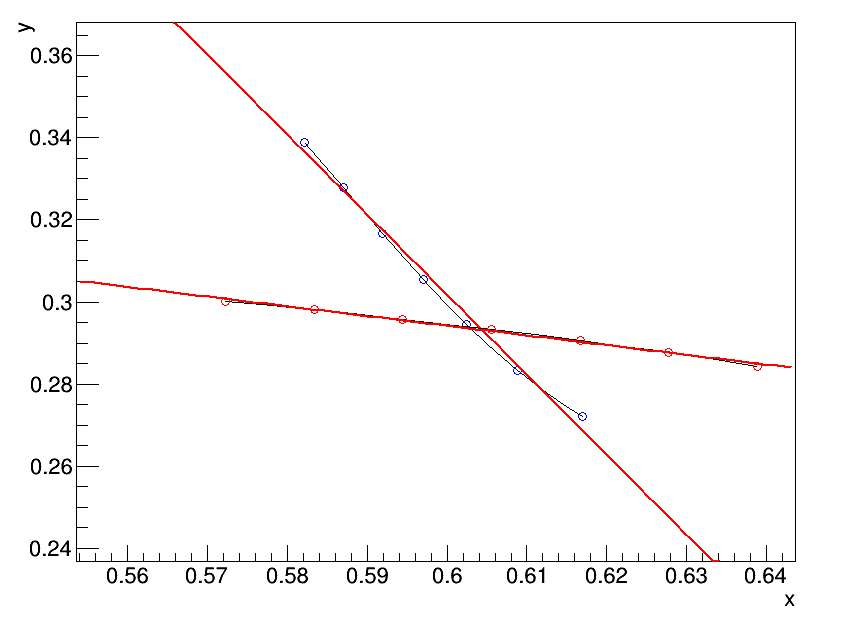
\includegraphics[width=0.80\linewidth]{cross}
\caption{convergence history of flow inside enclosed box for $\triangle t = 0.1$}
\label{cross}
\end{figure}


1 vortice
intercept x = 0.628863 y = 0.284613   40x120

intercept x = 0.607763 y = 0.291379   60x180

intercept x = 0.605327 y = 0.292402   70x210

intercept x = 0.605493 y = 0.292715   80x240

intercept x = 0.604404 y = 0.293177   90x270

2 vortice

intercept x = 0.614811 y = 1.352830   40x120

intercept x = 0.521546 y = 1.365390   60x180

intercept x = 0.518180 y = 1.367486   70x210

intercept x = 0.516247 y = 1.370399   80x240

intercept x = 0.515219 y = 1.371391   90x270

3 vortice

intercept x = 0.500413 y = 2.740107  40x120

intercept x = 0.496878 y = 2.732679  60x180

intercept x = 0.497183 y = 2.733485  70x210

intercept x = 0.497947 y = 2.727510  80x240

intercept x = 0.497706 y = 2.729092  90x270











\section{Conclusion}
This project provides great insight into the internal algorithms used for calculating numerical solutions for time varying problems. The Energy Equation applied to a steady state channel provided a great platform for developing and testing the program. Having the analytic solution really help fine tune the program and helped given an idea on how accurate the solutions could be. Investigating the error and how it changes relative to boundaries and mesh sizes will provides insight on how the methods should be applied to bigger problems to minimize time and error. Stability analysis provided a great means for understanding the computational limits of the program in terms of speed. Numerical methods provide a great way of solving difficult problems and until new methods are discovered for finding exact solution will remain the main method for finding solutions to difficult problems. 





\newpage
\appendix
\section{Appendix} \label{App:Appendix}
\subsection{Thomas Block Data Last Pass}
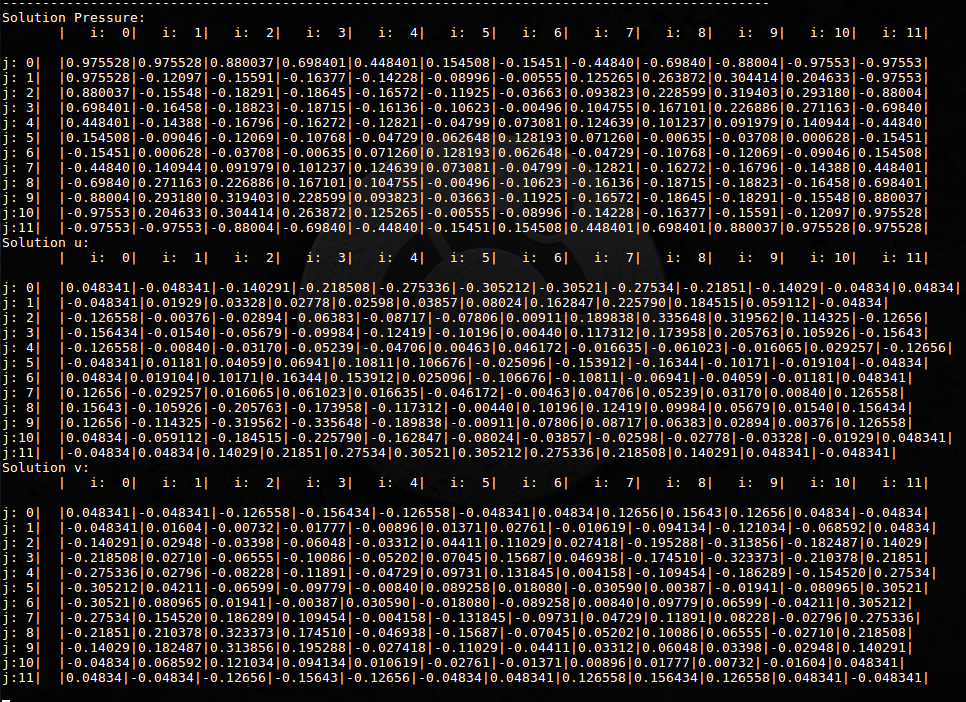
\includegraphics[width=0.95\linewidth]{tom}

\subsection{FinalProb.cpp}
\begin{lstlisting}




\end{lstlisting}

\begin{thebibliography}{99} % Beamer does not support BibTeX so references must be inserted manually as below
\bibitem[Celik, 2006]{p0}Ismail B. Celik1, Urmila Ghia, Patrick J.Roache and Christopher J. Freitas
\newblock "Procedure for Esitmation and Reporting Uncertainty Due to Discretization in CFD apllications",  West Virginia University, Morgantown WV, USA

\end{thebibliography}


%%% End document
\end{document}